\section{Hardware platforms}

\subsection{RFID - Radio frequency identification}

\begin{itemize}
		\item Passive tags get energy from received signal
		\item Active tags on-board battery
		\item Near-field communication: Data and power transmission via
				magnetic field to tag. Tag's data affects magnetic field, which
				is measured by RFID reader.
		\item Far-field communication: EM used to transfer power to tag, EM
				backscatter to send data from tag to RFID reader. Up to
				\SI{100}{\meter}
		\item NFC is a form of RFID at \SI{13.56}{\mega\Hz}, with two-way communication
\end{itemize}

\subsection{Sensor nodes}

\begin{description}
		\item[Energy-efficiency] Tradeoff: General-purpose hardware less efficient than embedded
				processors. ASICS inbetween.
		\item[Tiered network architecture] Sensor nodes with low computing
				resources, report to computing nodes which aggregate. Those to
				delivery nodes with high bandwith, which send to gateway nodes
				which are hooked up to the internet. Allows most nodes to be
				cheap, expensive operations to take place at nodes with static
				power supply.
		\item[Multi-processor nodse] Multiple simpler processors, flexibile
				energy saving by only turning on what's needed.
\end{description}

Classification of sensor node hardware:
\begin{description}
		\item[System-on-Chip]: RF (radio), CMOS (transistors), MEMS (mechanical
				system) on single chip. Low power, small nodes. Special
				instruction sets, limited support for reprogramming. Example: PicoNode.
		\item[Dedicated embedded nodes] Commerical OTS chip sets, low-power
				processing and communications. Full hardware access, C or ASM.
				Example: TelosB.
		\item[General-purpose computers] Based on PCs or PDAs, OTS OS and
				applications. Standard communication (bluetooth, wireless,
				...). High flexibility. Example: Raspberry Pi.
\end{description}


\subsection{Energy sources}

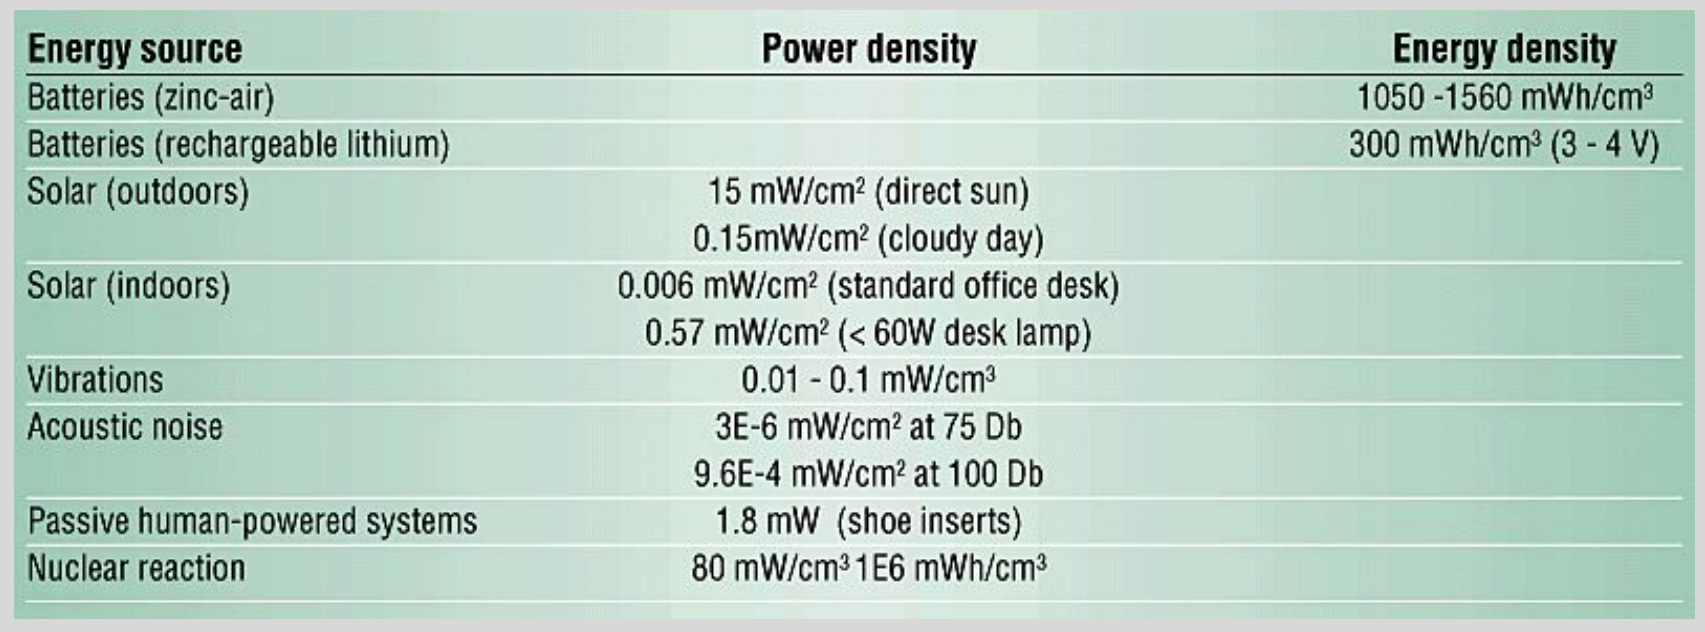
\includegraphics[width=\textwidth]{02_energy_sources}

\begin{description}
		\item[Energy scavenging] Photovolatic, temperature gradients, vibratinos, ...
\end{description}

\subsection{Energy saving in sleep mode}

Given power consumption active / sleep $P_{active}$ and $P_{sleep}$, $t_1$ time
when sleep mode entered, $t_{down}$ when fully powered down, $t_{event}$ when
waking up, then $E_{saved}$ energy saved, $E_{overhead}$ overhead due to sleep.
Sleep mode beneficial if $E_{saved} > E_{overhead}$. Where:

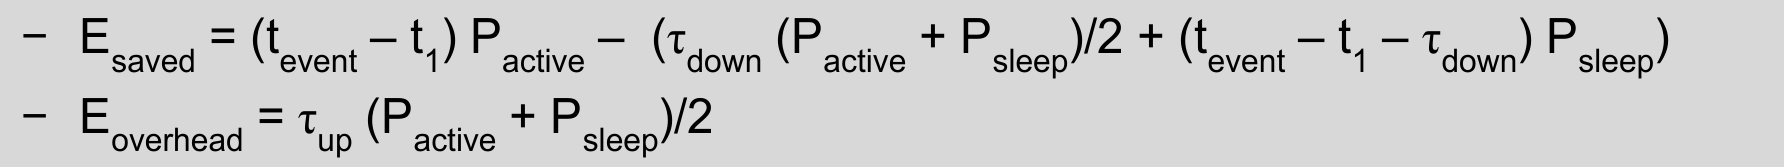
\includegraphics[width=\textwidth]{02_energy_saving}

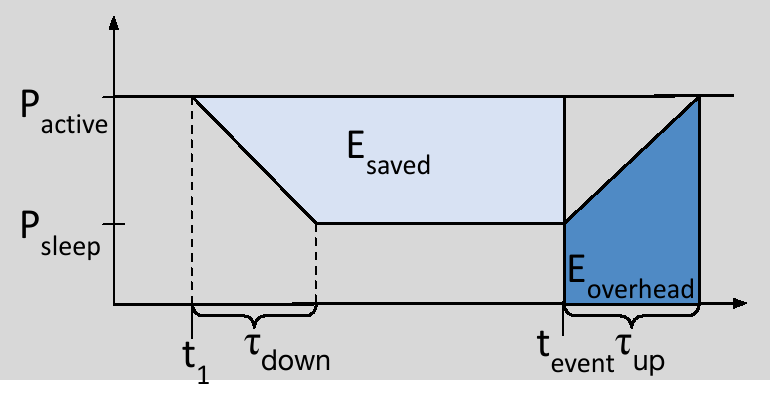
\includegraphics[width=0.5\textwidth]{02_energy_saving_model}

\subsection{Dynamic Voltage Scaling}

Switching power dissipated (= losses!) by capacitor is $P_{dynamic} = C \cdot F
\cdot V^2$, $C$ capacity, $F$ switching frequency, $V$ supply voltage. Dynamic
voltage scaling allows reducing power consumption in embedded system, by
reducing switching losses, by reducing voltage and frequency of processors.

\subsection{Transceiver}

\begin{itemize}
		\item Offers service (packet, byte, bit) to upper layer
		\item States: Transmit, receive, idle, sleep
		\item Handles modulation, coding, carrier-sensing, ...
		\item Often large startup time and cost when starting to send
		\item Ideally transmit few large packets instead of many small
\end{itemize}

\subsection{Multi-hop communication}

Energy cost over $d$ distance roughly $E \approx d^n$, where $n$ is path loss
factor of $2$ to $4$. Multi-hop communication can be way cheaper:

\begin{align*}
		E(h, d) = h \cdot(\alpha + \beta \cdot \frac{d}{h}^n)
\end{align*}

Where $\alpha$ sum of distant-independent components (eg receiver, startup,
...), $\beta$ distant-dependant terms eg power amplifier, path loss.
